%\documentclass[sigconf, authordraft]{acmart}
\documentclass[sigconf]{acmart}

\usepackage{booktabs} % For formal tables


% Copyright
%\setcopyright{none}
%\setcopyright{acmcopyright}
%\setcopyright{acmlicensed}
\setcopyright{rightsretained}
%\setcopyright{usgov}
%\setcopyright{usgovmixed}
%\setcopyright{cagov}
%\setcopyright{cagovmixed}


% DOI
\acmDOI{10.1145/3321707.3321726}

% ISBN
\acmISBN{978-1-4503-6111-8/19/07}

% Conference
\acmConference[GECCO '19]{the Genetic and Evolutionary Computation Conference 2019}{July 13--17, 2019}{Prague, Czech Republic}
\acmYear{2019}
\copyrightyear{2019}

%\acmArticle{4}
\acmPrice{15.00}

\begin{document}
\title[What\textquotesingle s inside the black-box? A GP method for interpreting complex ML models]{What\textquotesingle s inside the black-box? A genetic programming method for interpreting complex machine learning models}

%%% The submitted version for review should be ANONYMOUS
\author{Morgan Jones}
\affiliation{\institution{Department of Computer Science\\Aberystwyth University}}
\email{mwj7@aber.ac.uk}


\begin{abstract}
In this work, we present a new approach to interpretable machine learning; using multi-objective genetic programming to construct simple representations of complex black-box Machine learning models.
Our results are far simpler with comparable reconstructive performance than that of existing state-of-the-art methods.  Demonstrated on a range of datasets our resulting interpretable model (a single decision tree) approximates the knowledge of 200 layer neural networks and ensembles of 500 trees.
\end{abstract}

%
% The code below should be generated by the tool at
% http://dl.acm.org/ccs.cfm
% Please copy and paste the code instead of the example below. 
%
\begin{CCSXML}
<ccs2012>
<concept>
<concept_id>10011007.10011074.10011092.10011782.10011813</concept_id>
<concept_desc>Software and its engineering~Genetic programming</concept_desc>
<concept_significance>500</concept_significance>
</concept>
</ccs2012>
\end{CCSXML}

\ccsdesc[500]{Computing Methodologies~Genetic Programming}

\keywords{Explainable Artificial Intelligence, Interpretable Machine Learning, Evolutionary Multi-objective Optimisation}

\maketitle

\section{Introduction} 
Understanding the decisions behind Machine Learning (ML) techniques is important for their adoption into new areas where an AI\textquotesingle s decisions have greater consequences. This need for interpretability has created the push for explainable AI (XAI).

Traditional tree-based methods from XAI suffer from limitations, due to the greedy nature of the tree construction algorithms. Using Genetic Programming (GP) [19] we evolve trees, while simultaneously optimising our conflicting objectives of accuracy and simplicity, instead of constructing them in a greedy manner.

To the best of our knowledge GP has not been used for constructing IML models. In this work we propose a new multi-objective GP-based method for IML model extraction. Are objectives are:  
\begin{itemize}
  \item Propose a simple, human-readable tree structure which can be used for reconstructing complex predictions
  \item Simultaneously maximise the reconstruction ability while minimising the complexity of the trees
  \item Generate a frontier of trade-off solutions for user selection
  \item Evaluate the method against current state-of-the-art approaches on various datasets. 
\end{itemize}
The proposed method is applicable to any black-box (arbitrarily complex) classifier.

\section{The New Method}
In this section, a novel tree-based method is proposed for XAI. We use NSGAII [11], paired with strongly-typed GP (STGP) [24], to evolve decision tree-like structures, which simultaneously balance the complexity and the accuracy of the trees. Our goal is to outperform greedy methods, while still being computationally feasible. Another benefit of this approach is that a Pareto front of non-dominated trees is produced instead of just a single tree. This is useful for XAI as it allows a user to select a tree for visualisation at a desired complexity to accuracy trade-off point along the front.
\subsection{Overall Algorithm}
The overall training algorithm is shown in Fig. 1. The black-box classifier is trained once only on the original data (x and y values), then the evolutionary process is performed based on the resulting predictions (\^{y}) from this black-box model. The evolutionary algorithm never sees the original labels (y), as this is instead attempting to recreate the predicted labels (\^{y}). At the end of the evolutionary run, the result is a set of Pareto optimal models/trees which approximate the complex black-box model. Only the model with the highest reconstructive ability is used here. The overall evolutionary process is similar to NSGA-II. When selecting individuals, the non-dominated sorting in NSGA-II algorithm is used to rank the individuals, to ensure elitism this sorting is done across both the parent and child populations combined. 
\subsubsection{Objective Functions}
Two Objectives are:
\begin{itemize}
\item \textbf{Reconstruction ability} (\textit{maximisation}): The average weighted f1 metric as result of an internal (training set only) 3-fold (k=3) cross-validation on the tree
\end{itemize}
\begin{itemize}
\item \textbf{Complexity} (\textit{minimisation}): Number of splitting points (nodes) in the tree
\end{itemize}
Objective 1:
\begin{equation} \label{eq:obj1}
maximise \frac {1}{k} \sum_{i=1}^k f1(predict(fold(i)),blackbox\_predict(fold(i)))
\end{equation}
Where $f1$ is the weighted f1-score (weighted by the number of instances per class c)
\begin{displaymath}
f1(predicted, real) = (\sum_{c\in C} |C| \times \frac{2\times precision\times recall}{precision+recall})/\sum_{c\in C} |C|
\end{displaymath}
Objective 2:
\begin{equation}
minimise \sum split\_points
\end{equation}
\begin{figure}
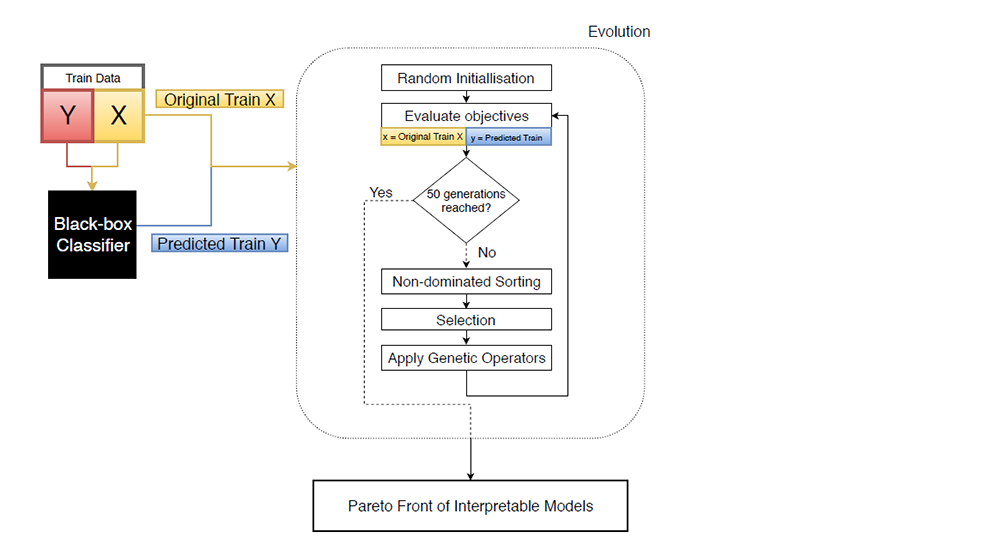
\includegraphics[width=0.75\textwidth]{evolution_process_resized}
\caption{Evolutionary Training Process.}
\end{figure}

\subsubsection{Representation}
The evolved trees are decision tree-like, meaning the input is at the root, the output at a leaf, and the internal nodes are splitting points. Traditionally with GP (parse-trees), the inputs are at the leaves (terminals), the output is at the root, and the internal nodes are functional components (functions). To get around this, data is passed in at the leaves but only functions are returned until the root node (only one branch will end up returning values for a given input), and then the functions are executed once we are at the root. For visualisation and use-cases, the two can be treated uniformly. 

Some simple patterns have needlessly complex representations in decision trees with axis-parallel splits. To solve this, the trees can construct features (as mathematical expressions) implicitly and check if those constructed features are greater than or equal to zero. For example: 
\begin{center}
Consider the condition if f1 >= f2 then class 1 else class 0. Without constructed features the resulting tree would be complex. With constructed features we can simply use one split as f1-f2>=0.
\end{center}

Using constructed features is beneficial to XAI because simpler rules are learnt.
\section{Experiments}
\subsection{Experiment Details}
\subsubsection{Datasets}
30 datasets from the OpenML repository [33] were used for comparison. These were the 20 most run binary datasets, and 10 most run multiclass datasets. The datasets were restricted to less than 15000 instances, less than 5 classes, and no missing values. These datasets are from a variety of domains, and have a varying number of features (both categorical and numeric), classes, and instances. The datasets offer a broad range to ensure generalisability of the proposed method.
\subsubsection{Comparison Methods}
Current state-of-the-art approaches to model extraction were trialled:
\begin{itemize}
\item Bayesian rule lists [35] (as pysbrl on pip)
\item A (h2o) decision tree [31]
\item A simplified (scikit-learn) [25] decision tree [22]
\item Logistic regression with L1-regularization (from scikit-learn)
\end{itemize}
Pre-Processing: One-hot-encoding was required for the scikit-learn methods to support categorical features. Multi-interval discretization is applied for the Bayesian rule lists to support continuous features.
\subsubsection{GP Parameter Settings}
The evolutionary search was run for 50 generations, with 100 trees in each generation. Trees were limited to a maximum height of 17. A crossover rate of 0.8 was used, and a mutation rate of 0.2. Top performing individuals are never lost, as the $\mu + \lambda$ algorithm [2] is used, with both values set to the population size (i.e. keep the 100 best).
\subsubsection{Evaluation Measures}
\paragraph{Classification Performance}
For measuring performance, we use a weighted f1-measure. For presentation we scale this to the range 0\ldots100.
\paragraph{Complexity}
We define complexity as the number of splitting points in the tree. If constructed features are used they count as multiple splits (f1+f2<=0 would count as 2). For Bayesian rule lists the complexity is measured as the number of rules + the number conjunctions in these rules. For logistic regression complexity is measured as the number of non-zero coefficients.
\subsubsection{Black-box Methods}
We chose three of the most common and high performing black-box models. All are implemented in h2o [31].
\begin{itemize}
\item Random Forests (with 500 trees)
\item Gradient Boosting (with 500 trees)
\item A deep neural network (200 hidden layers with 200 neurons each)
\end{itemize}
\textit{Note}: These methods were not finely tuned. Their relative performance is not of importance we are just trying to reconstruct their predictions.
\subsubsection{Significance Tests}
To compute whether the difference in reconstruction ability across datasets for each method was statistically significant, we used Friedman tests paired with Nemenyi post-hoc analysis.

To show the average reconstruction ability for each method we present the average accuracy of a 10-fold cross-validation, where each method gets the same train-test sets. The averages are also across the 3 black-box methods therefore for each method, 30 runs are executed for each of the 20 datasets. The goal is for the extraction methods to be invariant to the black-box model used, hence the averaging.
\subsection{Results}
We compare methods based on the number of times each method was dominated. Where domination is defined as another method achieves a simpler representation with the same (or improved) recreation ability. We cannot compare hypervolumes of frontiers as the comparison methods only return a single solution therefore we select the solution from our resultant frontier with the highest reconstruction ability to represent our methods performance.

GP (the proposed method) was not dominated on any of the datasets (Fig. 2). One caveat is that analysing the dominated counts alone is not a comprehensive indicator of performance, since both the simplest possible model (majority class) and the black-box model itself would never be dominated. Another argument is that since GP was the only method which simultaneously balanced these objectives, the measure can be seen as biased towards the proposed method. This is true, but also shows the usefulness of population-based techniques such as GP as they can effectively optimise multiple objectives simultaneously. This shows that multi-objective optimisation is a good choice for IML, as the objectives were optimised better than the existing approaches (in terms of dominance).
\begin{center}
\begin{figure}[h]
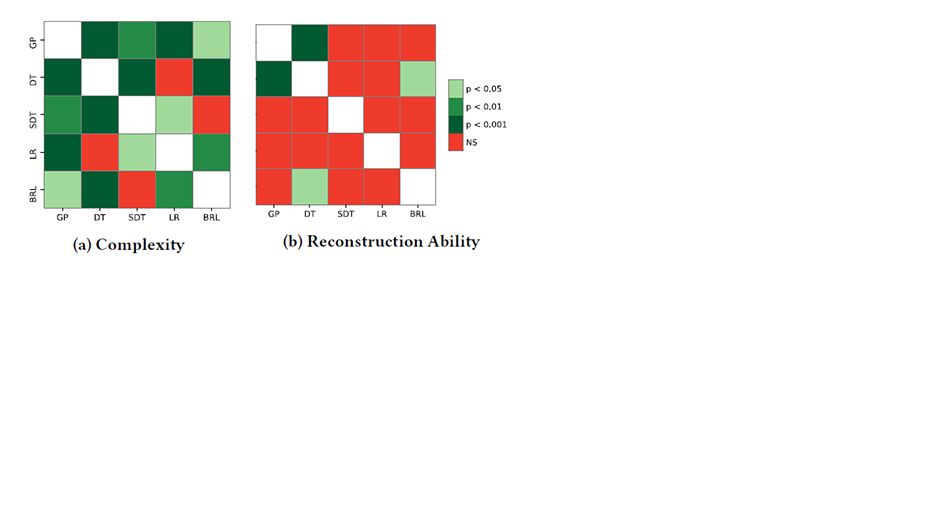
\includegraphics{result_analysis_resized}
\caption{Statistical significance testing.}
\end{figure}
\end{center}

Friedman testing paired with Nemenyi post-hoc analysis is performed to compare whether the difference in accuracies was statistically significant across datasets. The resulting p-values are visualised in Fig. 3.
\section{Further Analysis}
To give further insight into the resulting models from the compared IML methods, a comparison is given on the hill-valley dataset. The hill-valley dataset is considered the most challenging as the black-box models had lowest average test accuracy on this dataset. We can see that the proposed method\textquotesingle s resulting tree and the Bayesian rule list are by far the simplest interpretable models, both condense the 200 layer neural-network into small human readable form.

Looking further the Bayesian rule list just predicts 1 class so is considered overly simplistic. Looking into our evolved tree we can see its splitting points make sense when considering the hill-valley dataset, which "when plotted in order (from 1 through 100) as the Y coordinate, the points will create either a Hill (a `bump' in the terrain) or a Valley (a `dip' in the terrain)" [13]. We can see the tree is checking the first point, and comparing to the point at 30\% (i.e. the 30th feature), or the point at 70\%, where the tree is trying to distinguish between classes by finding the common points for the hills/valleys and checking if these are high or low relative to the training data (e.g. a high point at the start, a low point at 30\%, then a high point at 57\% indicates a valley based on this tree).

Below are the datasets that were most difficult for our method to reconstruct predictions for:
\begin{itemize}
\item The Autonuniv-Au7-500 and GesturePhase datasets have 5 classes. As the number of classes increases so does the complexity for tree-based methods. Here the push for smaller trees may need to be relaxed in cases where datasets contain a high number of classes.
\item Monks-Problems-2 is entirely categorical features. In the proposed method, a categorical node has a branch for each feature -- this potentially overfits to the training data. Combining categorical features into a single branch should be considered for future work.
\item For eeg-eye-state, the data is sequential/time-series. The proposed method is not optimised/designed for such datasets, so this explains the lower performance.
\end{itemize}
\section{CONCLUSIONS AND FUTURE WORK}
In this work, a novel model (agnostic) extraction method for XAI was proposed. Multi-objective GP is used to learn a simple and interpretable representation of a complex black-box model, which is often able to effectively reproduce the black-box\textquotesingle s predictions. This new method was compared to existing approaches for model extraction, and was found to offer drastically simpler models, with statistically equivalent test accuracy. To our best knowledge, this is the first utilisation of multi-objective optimisation in explainable AI. We also believe this is the first application of GP for model extraction, and shows a promising direction for future developments.

In future work we would like to focus on three main areas. Firstly, can recreation ability be improved without sacrificing simplicity? Secondly, can we find a more suitable measure of complexity to describe human interpretability?  And finally, is it possible to guide the evolution of the models based on human feedback?





\bibliographystyle{ACM-Reference-Format}
\bibliography{sample-bibliography} 

\end{document}
